% Source: Code/camera-to-radar_labeller/system_overview.tex
% Description: Object crossing scenario. Vessel A (Cargo, red) and Vessel B (Sailboat, blue) cross paths. Hungarian assignment may swap labels at the crossing point. JPDA and MHT maintain correct labels.

\documentclass[border=4pt]{standalone}
\usepackage{amsmath,amssymb,amsfonts}
\usepackage{tikz}
\usepackage{xcolor}
\usetikzlibrary{arrows.meta,positioning,calc,patterns,decorations.markings,shapes.geometric,fit,backgrounds}

\definecolor{Garnet}{HTML}{73000A}
\definecolor{Rose}{HTML}{CC2E40}
\definecolor{Atlantic}{HTML}{466A9F}
\definecolor{Congaree}{HTML}{1F414D}
\definecolor{Horseshoe}{HTML}{65780B}
\definecolor{Grass}{HTML}{CED318}
\definecolor{Honeycomb}{HTML}{A49137}
\definecolor{Black90}{HTML}{363636}
\definecolor{Black70}{HTML}{5C5C5C}
\definecolor{Black50}{HTML}{A2A2A2}
\definecolor{Black30}{HTML}{C7C7C7}
\definecolor{Black10}{HTML}{ECECEC}
\definecolor{WarmGrey}{HTML}{676156}
\definecolor{Sandstorm}{HTML}{FFF2E3}

\tikzset{
    every node/.style={font=\small},
    sysblock/.style={
        draw=Congaree, fill=Congaree!10, thick,
        minimum width=2.2cm, minimum height=1cm,
        align=center, sharp corners,
        text=black
    },
    sysarrow/.style={
        -Stealth, thick, color=Garnet
    },
    timeblock/.style={
        draw=none, fill=#1, minimum height=0.5cm,
        sharp corners, text=white, font=\footnotesize\bfseries,
        inner sep=2pt
    },
    ppiblob/.style={
        fill=#1, sharp corners, minimum size=4pt, inner sep=0pt
    },
}

\begin{document}
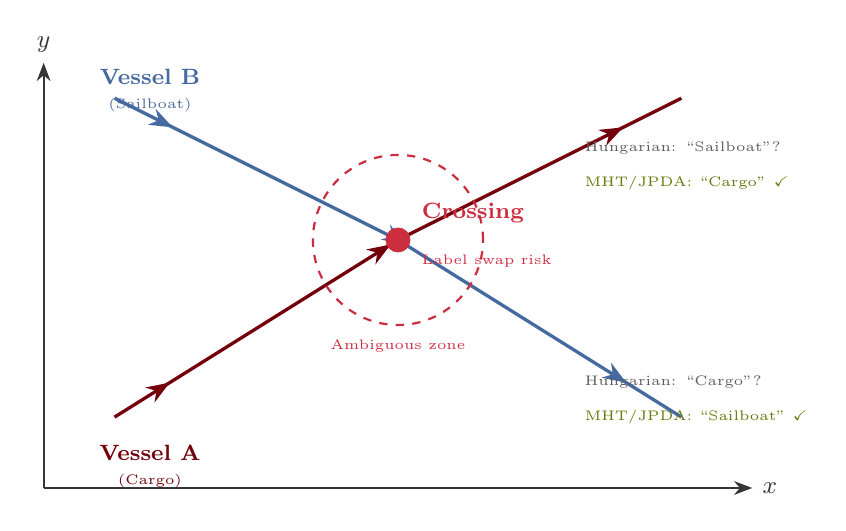
\begin{tikzpicture}[scale=0.9]
    % Time axis
    \draw[-Stealth, thick, color=Black90] (0,0) -- (10,0) node[right] {$x$};
    \draw[-Stealth, thick, color=Black90] (0,0) -- (0,6) node[above] {$y$};

    % Vessel A trajectory
    \draw[very thick, Garnet, decoration={markings,
        mark=at position 0.1 with {\arrow{Stealth}},
        mark=at position 0.5 with {\arrow{Stealth}},
        mark=at position 0.9 with {\arrow{Stealth}}},
        postaction={decorate}]
        (1,1) -- (5,3.5) -- (9,5.5);
    \node[font=\footnotesize\bfseries, text=Garnet] at (1.5,0.5) {Vessel A};
    \node[font=\tiny, text=Garnet] at (1.5,0.1) {(Cargo)};

    % Vessel B trajectory
    \draw[very thick, Atlantic, decoration={markings,
        mark=at position 0.1 with {\arrow{Stealth}},
        mark=at position 0.5 with {\arrow{Stealth}},
        mark=at position 0.9 with {\arrow{Stealth}}},
        postaction={decorate}]
        (1,5.5) -- (5,3.5) -- (9,1);
    \node[font=\footnotesize\bfseries, text=Atlantic] at (1.5,5.8) {Vessel B};
    \node[font=\tiny, text=Atlantic] at (1.5,5.4) {(Sailboat)};

    % Crossing point
    \fill[Rose] (5,3.5) circle (5pt);
    \node[font=\footnotesize\bfseries, text=Rose, above right] at (5.2,3.6) {Crossing};
    \node[font=\tiny, text=Rose, right] at (5.2,3.2) {Label swap risk};

    % Danger zone
    \draw[Rose, thick, dashed] (5,3.5) circle (1.2cm);
    \node[font=\tiny, text=Rose] at (5,2.0) {Ambiguous zone};

    % Post-crossing labels (wrong)
    \node[font=\tiny, text=Black70, right] at (7.5,4.8) {Hungarian: ``Sailboat''?};
    \node[font=\tiny, text=Black70, right] at (7.5,1.5) {Hungarian: ``Cargo''?};

    % Post-crossing labels (correct)
    \node[font=\tiny, text=Horseshoe, right] at (7.5,4.3) {MHT/JPDA: ``Cargo'' \checkmark};
    \node[font=\tiny, text=Horseshoe, right] at (7.5,1.0) {MHT/JPDA: ``Sailboat'' \checkmark};
\end{tikzpicture}
\end{document}
